\section{Equivalence} \label{chapter4:equivalence}

The goal of this thesis is not to propose a new high-level language but to automate the architectural shift.
The next paragraphs introduces the equivalence between the memory abstraction of the event-driven execution model and of the pipeline architecture previously presented.
The equivalence is broken down in two steps, as illustrated in figure \ref{fig:chapter4:roadmap}.
The first step identifies the stages of the pipeline and the rupture points between them in the control flow.
The second step enforces isolation of memory between these stages to preserve invariance.

\begin{figure}[h!]
\begin{center}
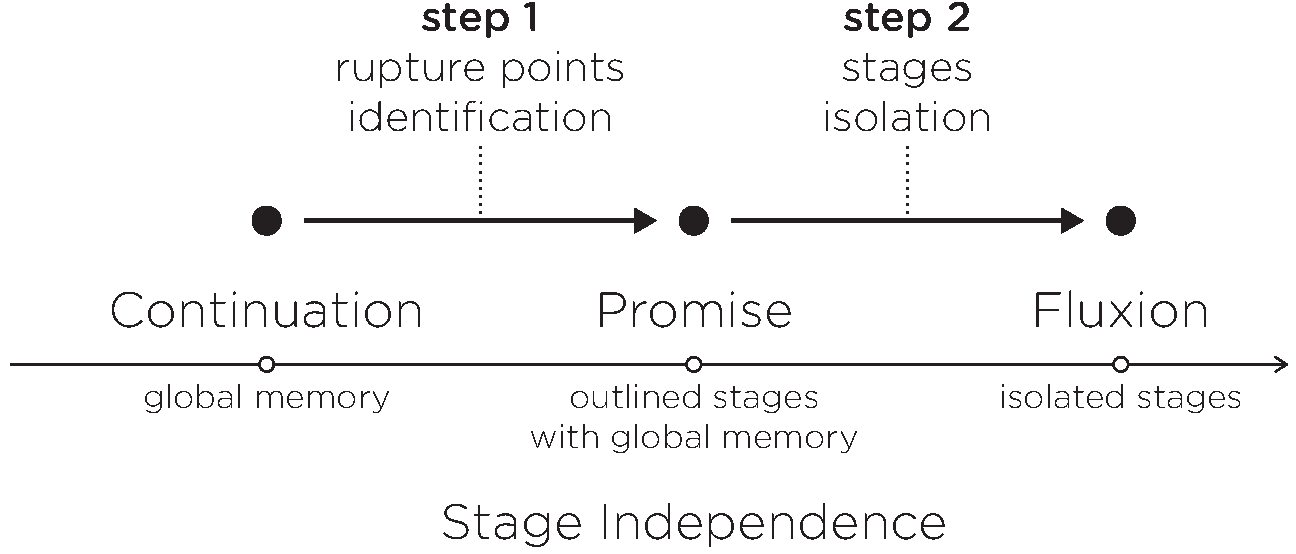
\includegraphics[width=0.9\textwidth]{../resources/roadmap.pdf}
\end{center}
\caption{Roadmap}
\label{fig:roadmap}
\end{figure}

\subsection{Rupture Point}

The pipeline architecture enforces the memory isolation between stages.
Each stage has its own thread of execution, and is independent from the others.
On the other hand, the execution flow of the event-loop jumps from one concurrent task to the other.
%  because of the continuation passing style and the common memory store.
% The message passing linking the callbacks is transparently handled by the event-loop.
However, the executions of these tasks are as distinct as the execution of the different stages of a pipeline.
The call stacks of two concurrent tasks are distinct.
The asynchronous function call between the caller and its continuation represents the rupture between two call stacks.
It is a rupture point, and is equivalent to a data stream between two stages in the pipeline architecture.

Both the pipeline architecture and the event-loop present these rupture points.
The detection of rupture points allows to map a pipeline architecture onto the implementation following the event-loop model.
To allow the transformation from one to the other, this thesis studies the possibility to detect rupture points, and to distribute the global memory into the parts defined by these rupture points.

The detection of rupture points is addressed in chapter \ref{chapter5}.
It presents the extraction of a pipeline of concurent tasks from a Javascript application.
Such pipeline is similar to the one exposed by Promises.
% The chapter proposes a simpler alternative to the latter called Dues.
However, these concurent tasks still require a global memory.
They can't be executed in parallel.

\subsection{Invariance}

% This transformation is important on two points.
% The conservation of the invariance.
% The equivalence between the coordinations.

The global memory assures the total ordering of tasks, and requires sequentiality, while message passing assures causal ordering of tasks and allows parallelism.
The causal ordering of tasks, by opposition to total ordering, is sufficient to assure the correctness of the execution.
Therefore, to assure the correctness of the execution, the ordering allowd by the global memory is partially equivalent to message passing ordering.
And it is possible to transform the global memory coordination into message passing.
% Given that the tasks are independent and communicate by messages.

% This result was used by Lamport to prove the correctness of distributed systems.
Yet, to preserve the correctness as expressed by the developer, it is important to preserve the invariance.
The global memory needs not to be distributed into each of the stages of the pipeline, so that each stage have an exclusive access to its memory.

To assure the missing coordinations assured by the shared memory between the stages, the transformation should provide equivalent coordination with message passing.
The isolation and replacement of the global memory is addressed in chapter \ref{chapter6}, with the introduction of isolated containers called Fluxions.




% The invariance holds for the whole memory during the execution of each callback.
% As I explained in the previous section, this invariance is required to allow the concurrent execution of the different tasks.
% On the other hand, the invariance is explicit in the pipeline architecture, as all the stages have isolated memories.
% The coordination between these isolated process is made explicit by the developer through message passing.

% I argue that the state coordination between the callbacks requireing a global memory could be replaced by the message passing coordination used manually in the pipeline architecture.
% I argue that not all applications need concurrent access on the state, and therefore, need a shared memory.
% % Specifically, I argue that each state region remains roughly local to a stage during its modification.
% \nt{TODO review that, I don't know how to formulate these paragraphs. Identify the state and the data in the global memory.}

% \subsubsection{Transformation}

% This equivalence should allow the transformation of an event loop into several parallel processes communicating by messages.
% In this thesis, I study the static transformation of a program, but the equivalence should also hold for a dynamic transformation.
% I present the analyzis tools I developed to identify the state and the data from the global memory.